\documentclass[11pt, a4paper]{article}

\usepackage[utf8]{inputenc}
\usepackage[T1]{fontenc}
\usepackage{amsmath, amssymb}
\usepackage{booktabs}
\usepackage{graphicx}
\usepackage{hyperref}
\usepackage[margin=2.2cm]{geometry}
\usepackage{xcolor}
\usepackage{tcolorbox}
\usepackage{float}
\usepackage{enumitem}
\usepackage{multicol}

\definecolor{probcolor}{RGB}{41, 98, 163}
\definecolor{anscolor}{RGB}{163, 52, 41}
\definecolor{intcolor}{RGB}{41, 130, 72}

\newtcolorbox{problembox}{
    colback=probcolor!5!white,
    colframe=probcolor!70!black,
    fonttitle=\bfseries\sffamily,
    title={The Problem},
    arc=2pt, boxrule=0.8pt
}
\newtcolorbox{answerbox}{
    colback=anscolor!5!white,
    colframe=anscolor!70!black,
    fonttitle=\bfseries\sffamily,
    title={What We Built},
    arc=2pt, boxrule=0.8pt
}
\newtcolorbox{interpbox}{
    colback=intcolor!5!white,
    colframe=intcolor!70!black,
    fonttitle=\bfseries\sffamily,
    title={How to Read This},
    arc=2pt, boxrule=0.8pt
}

\newcommand{\VaR}{\operatorname{VaR}}
\newcommand{\ES}{\operatorname{ES}}

\title{%
    \vspace{-1cm}
    {\LARGE\sffamily\bfseries Risk Analyst: Portfolio Showcase} \\[0.4em]
    {\large\sffamily Frontier Quantitative Risk Analysis in Python} \\[0.3em]
    {\normalsize\sffamily 4 Projects $\cdot$ 67 Tests $\cdot$ 8{,}000+ Lines of Production Code}
}
\author{Andr\'es Gonz\'alez Ortega}
\date{\today}

\begin{document}
\maketitle
\thispagestyle{empty}

\noindent
This document presents the key outputs from four quantitative risk analysis projects.
Each section states the business problem, shows the solution, and explains how to interpret the results.
All code is open source at \texttt{github.com/GonorAndres/risk-analyst}.

\vspace{0.5em}
\hrule
\vspace{1em}

%% ============================================================================
\section*{Project 01 --- Portfolio Risk Dashboard}
%% ============================================================================

\begin{problembox}
A portfolio manager holds five assets (US equities, Nasdaq, small-caps, Treasuries, gold).
Every morning they need a number: \emph{``What is the most I could lose today?''}
And quarterly, they need to know: \emph{``Has my risk model been accurate?''}
\end{problembox}

\begin{answerbox}
We compute Value-at-Risk (VaR) and Expected Shortfall (ES) using three methods: historical simulation, parametric (normal), and Monte Carlo.
Then we backtest the model over 252 rolling days using the Kupiec test (unconditional coverage), the Christoffersen test (violation independence), and the Basel traffic-light system.
\end{answerbox}

\begin{figure}[H]
    \centering
    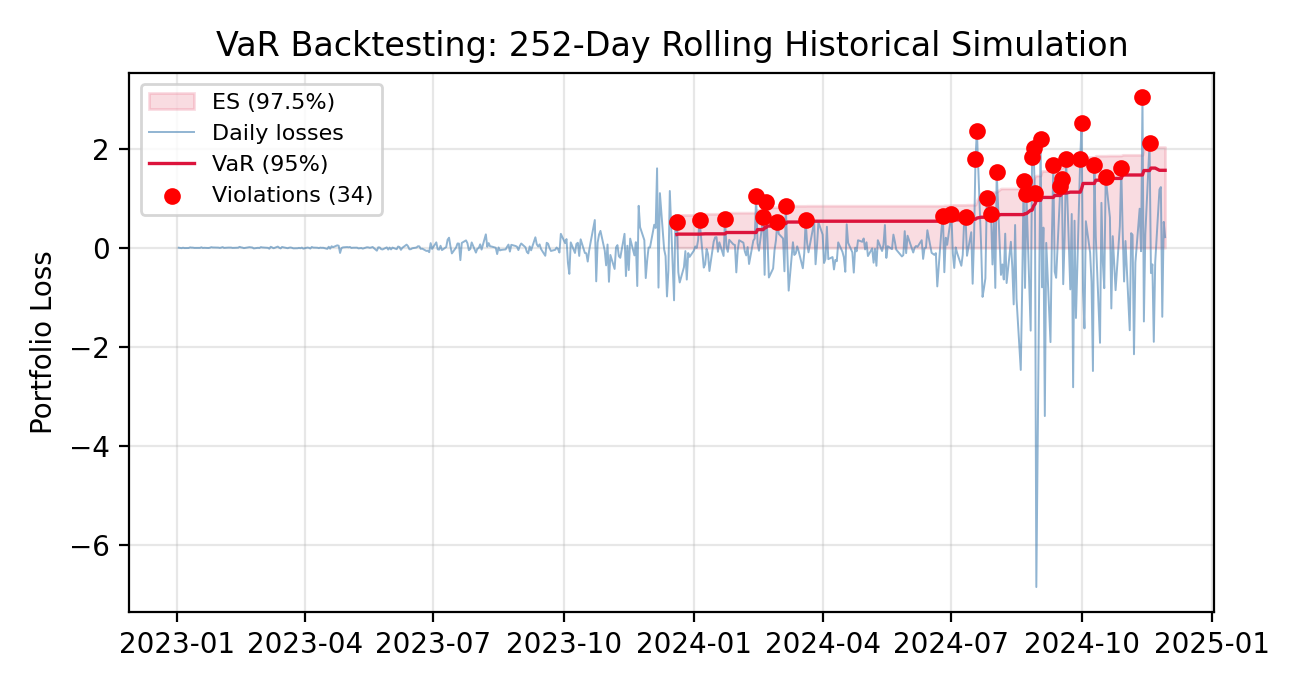
\includegraphics[width=\textwidth]{figures/p01_var_backtest.png}
    \caption{Rolling 252-day VaR backtest. Red dots mark days where actual losses exceeded the VaR forecast. The shaded region shows Expected Shortfall --- the average loss in the tail.}
\end{figure}

\begin{interpbox}
\textbf{VaR line (red)}: On any given day, we expect losses to stay below this line 95\% of the time.
When a red dot appears above the line, the model was wrong that day.

\textbf{Violation count}: At 95\% confidence over 248 days, we expect $\sim$12 violations.
If we see significantly more, the Kupiec test rejects the model (p-value $< 0.05$) and Basel assigns a yellow or red zone, which triggers higher capital requirements.

\textbf{ES shading}: The light red region shows that even when VaR is breached, losses average to ES --- roughly 1.5--2x the VaR threshold. This is the number regulators care about under Basel III/IV (FRTB).
\end{interpbox}

\begin{figure}[H]
    \centering
    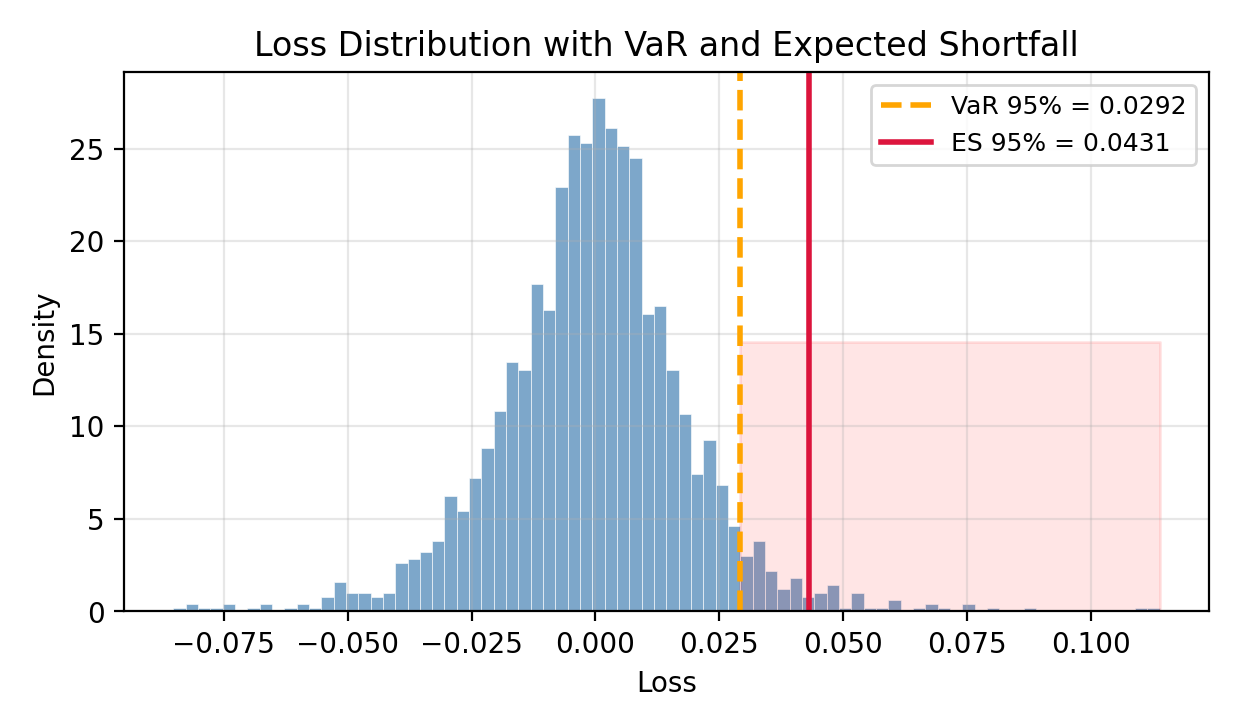
\includegraphics[width=\textwidth]{figures/p01_loss_dist.png}
    \caption{Loss distribution with VaR (dashed orange) and ES (solid red) marked. The shaded tail beyond VaR is where Expected Shortfall averages over.}
\end{figure}

\begin{interpbox}
The histogram shows that the loss distribution has heavy tails --- the right side extends much further than a normal distribution would predict.
VaR is just the 95th percentile cutoff (``losses won't exceed this 95\% of the time''), while ES averages over everything beyond that cutoff (``when things go wrong, they go \emph{this} wrong on average'').
ES is always $\geq$ VaR. The gap between them reveals how severe tail losses are.
\end{interpbox}

\newpage

%% ============================================================================
\section*{Project 02 --- Monte Carlo Simulation Engine}
%% ============================================================================

\begin{problembox}
Many risk calculations --- portfolio VaR for non-linear instruments, option pricing, stress testing --- have no closed-form solution.
We need to simulate thousands of possible futures and measure risk from the resulting distribution.
The challenge: naive simulation is slow and imprecise.
\end{problembox}

\begin{answerbox}
We built a reusable Monte Carlo engine that simulates correlated asset paths via Geometric Brownian Motion with Cholesky-decomposed correlation.
It prices European, Asian, and barrier options, and implements variance reduction techniques (antithetic variates, control variates) that cut standard error by 2--4x.
\end{answerbox}

\begin{figure}[H]
    \centering
    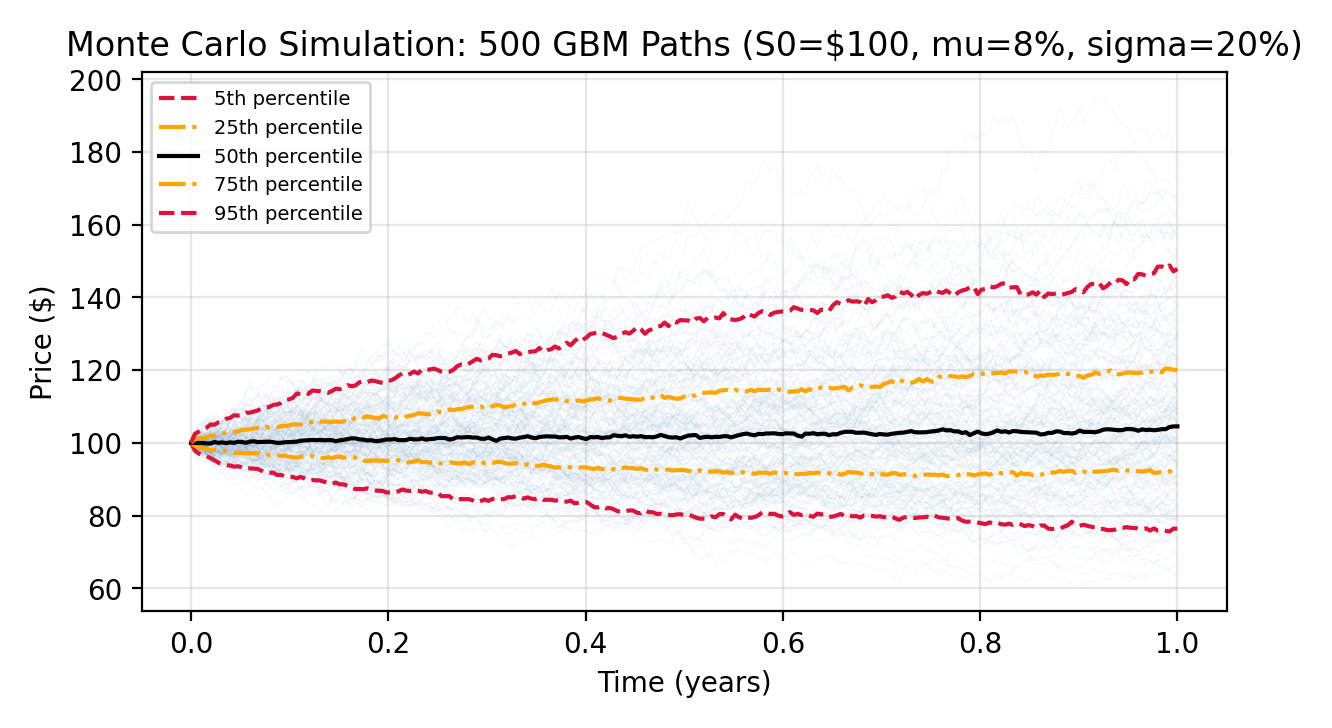
\includegraphics[width=\textwidth]{figures/p02_mc_paths.png}
    \caption{500 simulated GBM price paths from \$100 with $\mu = 8\%$, $\sigma = 20\%$. Percentile lines show the distribution of outcomes at each time step.}
\end{figure}

\begin{interpbox}
Each faint blue line is one possible future for the asset price.
The \textbf{black median line} shows the most likely outcome.
The \textbf{5th/95th percentile lines} (outer red dashes) bound the 90\% probability fan --- prices will land between these lines 90\% of the time.

Notice the fan widens over time: uncertainty grows with the square root of time.
After one year, the 90\% range spans roughly \$70--\$150 from a \$100 start.
This is the fundamental reason risk increases with holding period.
\end{interpbox}

\begin{figure}[H]
    \centering
    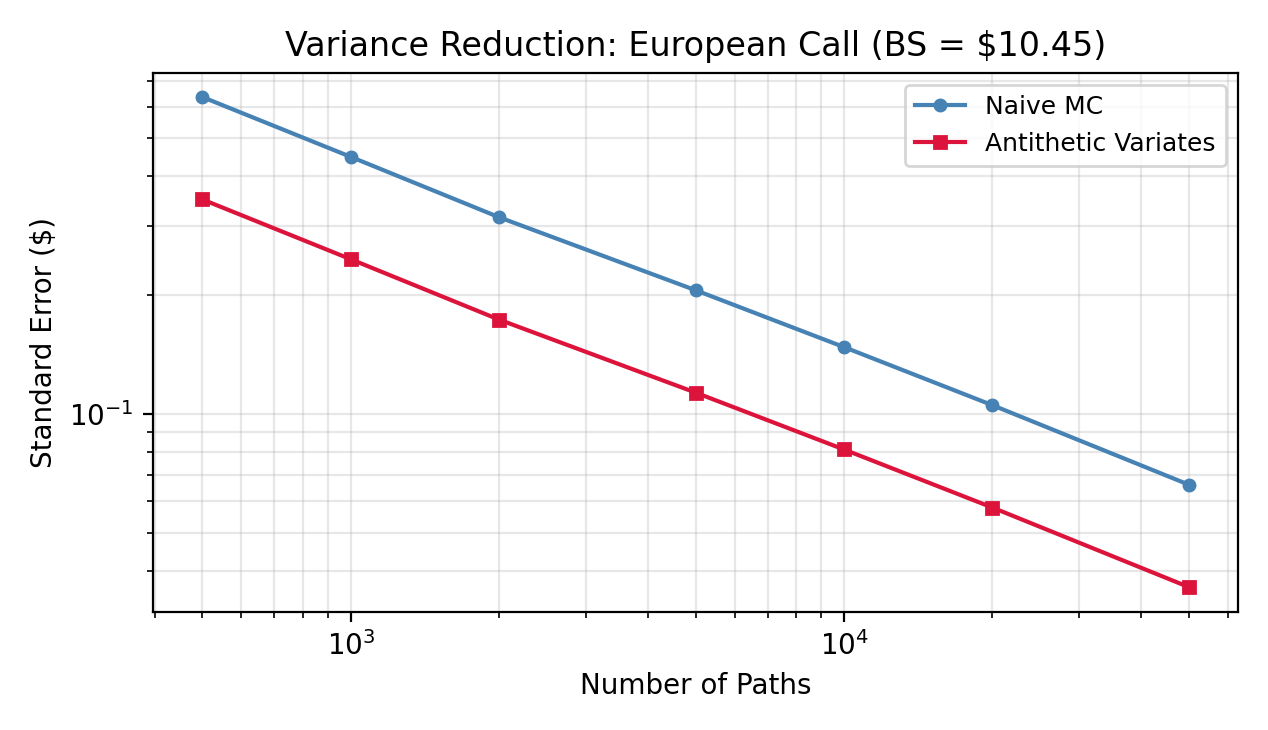
\includegraphics[width=\textwidth]{figures/p02_variance_reduction.png}
    \caption{Standard error of European call price estimate vs.\ number of simulation paths. Antithetic variates achieve the same precision with roughly 3x fewer paths.}
\end{figure}

\begin{interpbox}
Both lines slope downward: more simulations = more precision.
But the \textbf{antithetic variates line (red)} is consistently below the naive line (blue), meaning it achieves the same accuracy with far fewer simulations.

In practice, this means a VaR calculation that takes 10 minutes with naive MC can be done in 3 minutes with antithetic variates --- same precision, less compute.
For production risk systems running thousands of calculations per day, this efficiency gain is critical.
\end{interpbox}

\newpage

%% ============================================================================
\section*{Project 03 --- Credit Scoring with Machine Learning}
%% ============================================================================

\begin{problembox}
A bank receives 1{,}000 loan applications per day.
For each one: \emph{what is the probability this borrower will default?}
The answer determines loan approval, pricing, and capital reserves.
Regulators require the model to be \emph{explainable} --- a rejected applicant has the right to know why.
\end{problembox}

\begin{answerbox}
We built two PD (probability of default) models --- logistic regression with WoE-encoded features (interpretable) and gradient boosting (high-performance) --- on synthetic consumer lending data.
We evaluate with AUC, KS statistic, and Gini coefficient, and use SHAP values for explainability.
A full SR~11-7 model card documents the model for regulatory review.
\end{answerbox}

\begin{figure}[H]
    \centering
    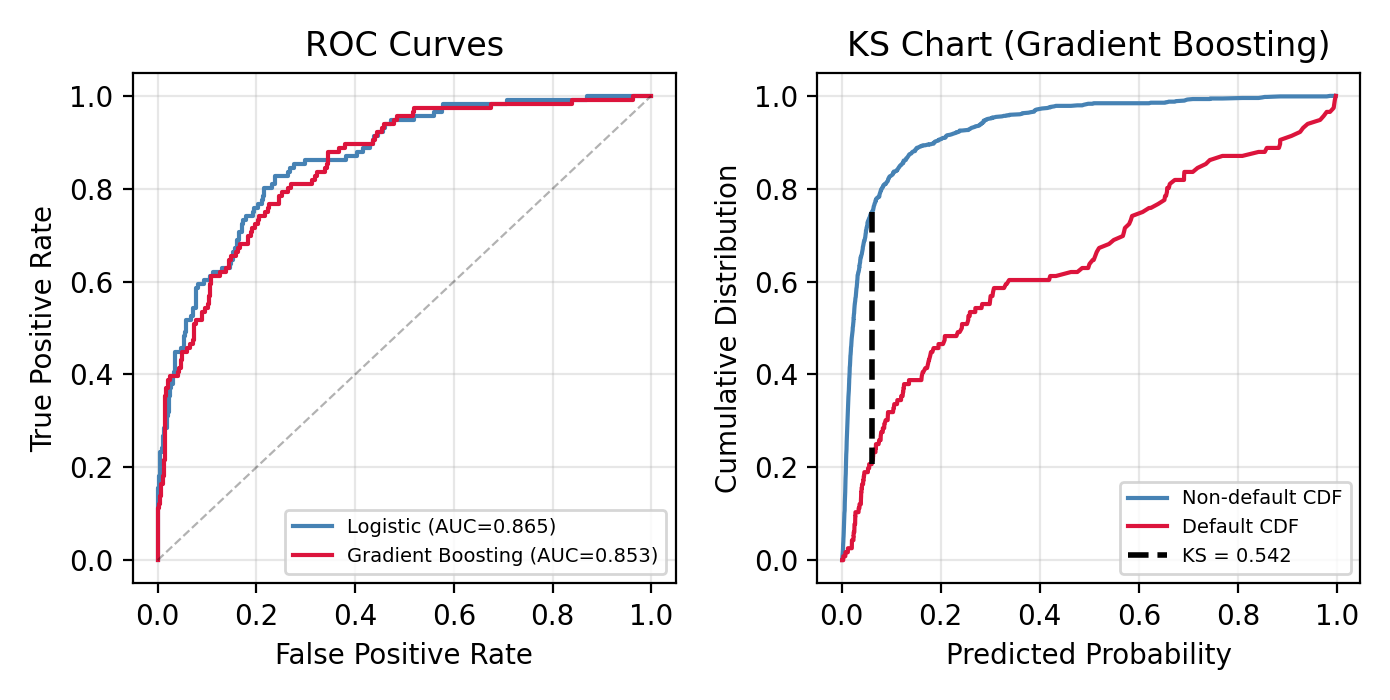
\includegraphics[width=\textwidth]{figures/p03_roc_ks.png}
    \caption{Left: ROC curves comparing logistic regression (AUC = 0.865) and gradient boosting (AUC = 0.853). Right: KS chart showing maximum separation between default and non-default distributions.}
\end{figure}

\begin{interpbox}
\textbf{ROC curve} (left): The further the curve bows toward the upper-left corner, the better the model separates defaulters from non-defaulters.
An AUC of 0.86 means the model correctly ranks a random defaulter above a random non-defaulter 86\% of the time.
Both models significantly outperform random chance (diagonal line).

\textbf{KS chart} (right): The vertical black line marks the point of maximum separation between the cumulative distributions of defaults and non-defaults.
A KS statistic of $\sim$0.55 indicates strong discriminatory power --- the model's predicted probabilities effectively sort borrowers by risk.

\textbf{Key insight}: the simpler logistic regression slightly outperforms gradient boosting here because WoE encoding pre-processes features into an optimal form for linear models.
In production, both would be maintained as challenger models per SR~11-7 guidelines.
\end{interpbox}

\begin{figure}[H]
    \centering
    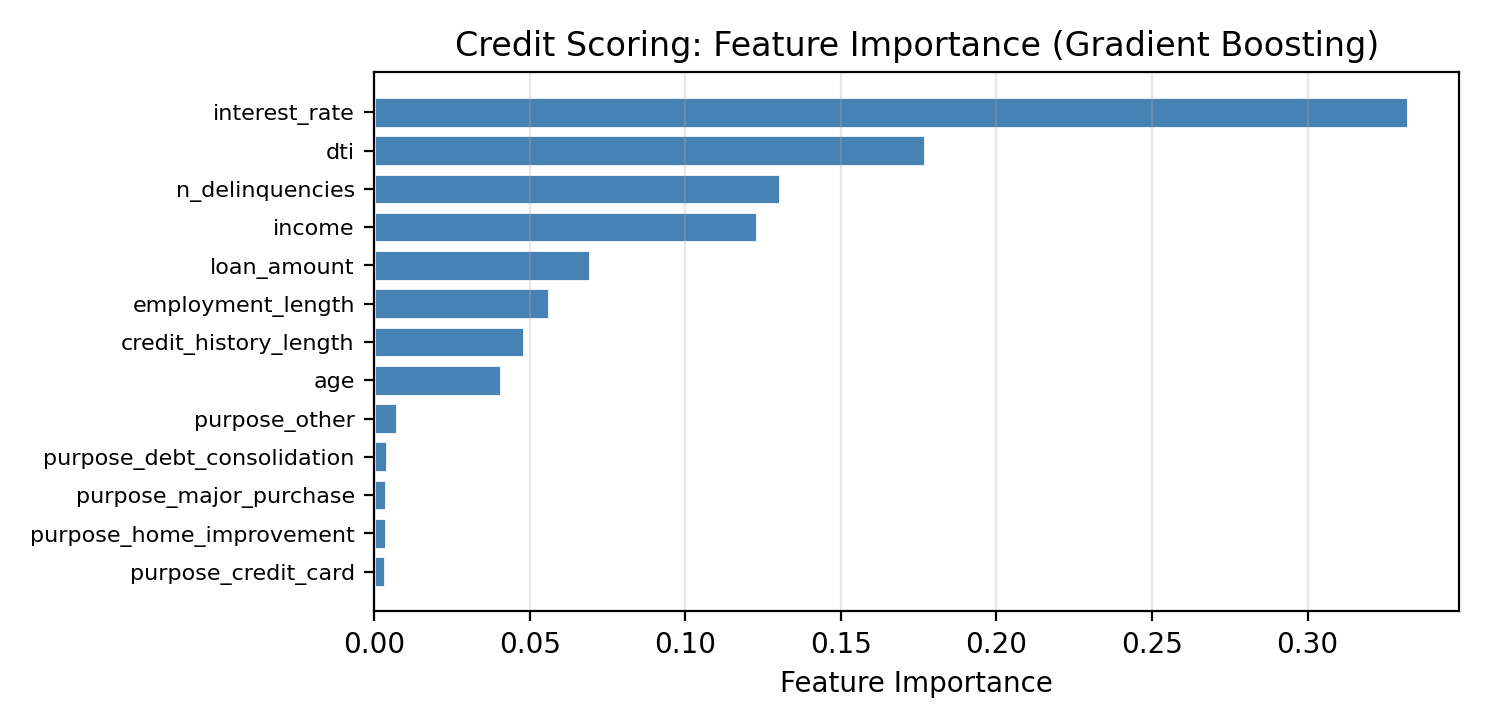
\includegraphics[width=\textwidth]{figures/p03_feature_importance.png}
    \caption{Feature importance from the gradient boosting model. The top predictors are income, delinquency history, and debt-to-income ratio.}
\end{figure}

\begin{interpbox}
This chart answers the regulator's question: \emph{``What drives the model's decisions?''}
The most important features (income, number of delinquencies, DTI ratio) align with economic intuition --- borrowers with lower income, past delinquencies, or high debt loads are riskier.

For individual decisions (``why was \emph{this} applicant rejected?''), we use SHAP waterfall plots that decompose each prediction into per-feature contributions.
This satisfies both SR~11-7 model governance and EU AI Act transparency requirements.
\end{interpbox}

\newpage

%% ============================================================================
\section*{Project 04 --- Volatility Modeling}
%% ============================================================================

\begin{problembox}
Standard risk models assume volatility is constant.
In reality, volatility \emph{clusters}: turbulent days breed more turbulent days, and calm periods persist.
A constant-volatility VaR model overestimates risk in calm markets (wasting capital) and underestimates it during crises (dangerous).
\end{problembox}

\begin{answerbox}
We fit GARCH(1,1), GJR-GARCH, and EGARCH models that capture time-varying volatility and the leverage effect (bad news increases volatility more than good news).
We also fit a Markov regime-switching model that identifies ``calm'' and ``crisis'' market states.
The fitted volatility feeds directly into conditional VaR/ES for more accurate risk estimates.
\end{answerbox}

\begin{figure}[H]
    \centering
    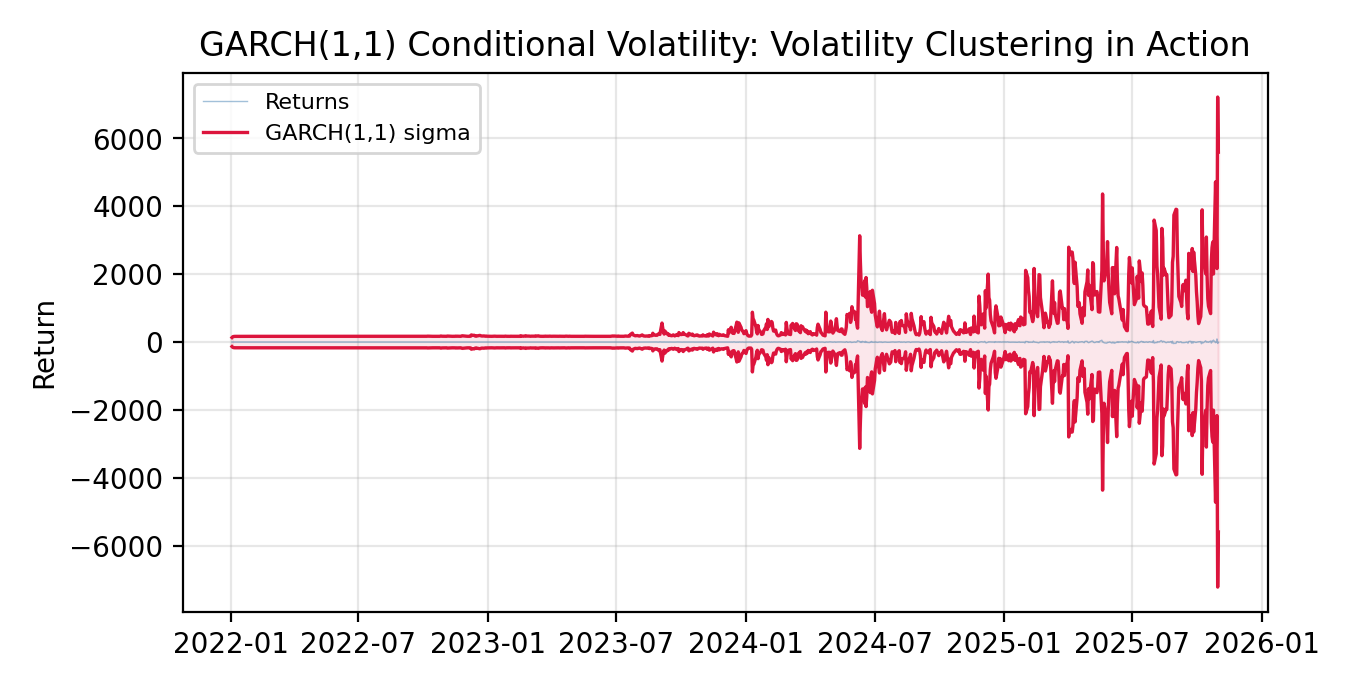
\includegraphics[width=\textwidth]{figures/p04_garch_vol.png}
    \caption{GARCH(1,1) conditional volatility (red envelope) overlaid on simulated returns. The envelope widens during turbulent periods and contracts during calm ones.}
\end{figure}

\begin{interpbox}
The \textbf{red envelope} is the GARCH model's real-time estimate of volatility.
When a large return occurs (positive or negative), the envelope widens because the model expects continued turbulence.
During quiet periods, it contracts.

This is the \textbf{volatility clustering} phenomenon: the autocorrelation of squared returns.
With typical S\&P\,500 parameters ($\alpha \approx 0.09$, $\beta \approx 0.90$), volatility shocks have a half-life of roughly 70 trading days --- a crisis doesn't just spike volatility, it keeps it elevated for months.

\textbf{Impact on risk}: During the wide-envelope periods, GARCH-based VaR correctly increases, while a constant-volatility model would remain flat and dangerously understated.
\end{interpbox}

\begin{figure}[H]
    \centering
    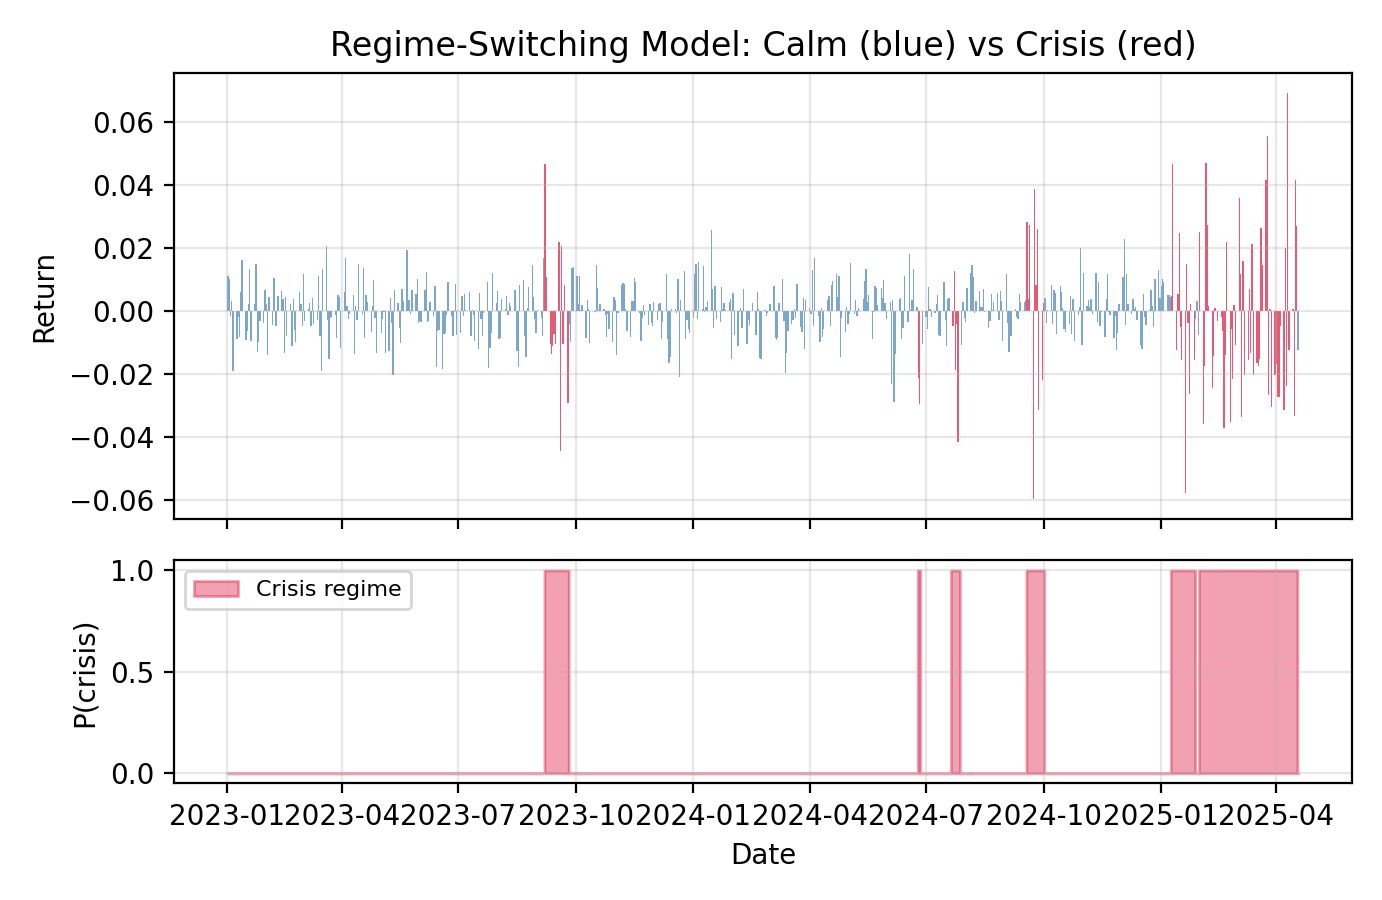
\includegraphics[width=\textwidth]{figures/p04_regime.png}
    \caption{Regime-switching model: returns colored by detected regime (blue = calm, red = crisis). Bottom panel shows the probability of being in the crisis state.}
\end{figure}

\begin{interpbox}
The regime-switching model takes a different approach: instead of smoothly varying volatility, it assumes the market flips between two distinct states with different risk profiles.

\textbf{Top panel}: Returns are color-coded by regime. Crisis periods (red) show larger, more volatile swings. The model detects these shifts automatically from the data.

\textbf{Bottom panel}: The filtered probability of being in the crisis regime. When this probability spikes to 1.0, the model is confident the market has entered a high-volatility regime.
Risk managers can use this as an early warning system: when crisis probability exceeds 0.5, switch to conservative positions or increase hedging.

\textbf{Transition dynamics}: The model estimates that calm periods persist ($p_{11} \approx 0.98$, expected duration $\sim$50 days) while crises are shorter-lived ($p_{22} \approx 0.93$, expected duration $\sim$14 days).
\end{interpbox}

\vspace{1em}
\hrule
\vspace{1em}

%% ============================================================================
\section*{Technical Summary}
%% ============================================================================

\begin{center}
\begin{tabular}{@{}clcl@{}}
\toprule
\textbf{\#} & \textbf{Project} & \textbf{Tests} & \textbf{Key output} \\
\midrule
01 & Portfolio Risk Dashboard     & 36 & VaR/ES backtesting with Kupiec, Christoffersen, Basel \\
02 & Monte Carlo Engine           & 17 & Correlated simulation with variance reduction \\
03 & Credit Scoring with ML       & 14 & PD model with AUC = 0.86, SHAP explainability \\
04 & Volatility Modeling           & 14 & GARCH family + regime-switching \\
\addlinespace
   & \textbf{Total}               & \textbf{67} & \textbf{8{,}000+ lines of tested, typed Python} \\
\bottomrule
\end{tabular}
\end{center}

\medskip

\noindent
\textbf{Stack}: Python 3.11+, NumPy, SciPy, pandas, scikit-learn, XGBoost, arch, statsmodels, matplotlib.

\noindent
\textbf{Standards}: SR~11-7 model governance, Basel III/IV FRTB alignment, full type hints, pytest with property-based testing.

\noindent
\textbf{Repository}: \texttt{github.com/GonorAndres/risk-analyst} --- MIT License.

\vfill
\hrule
\smallskip
\noindent\textit{Andr\'es Gonz\'alez Ortega --- UNAM Actuarial Science} \hfill \textit{\today}

\end{document}
